\let\negmedspace\undefined
\let\negthickspace\undefined
\documentclass[journal]{IEEEtran}
\usepackage[a5paper, margin=10mm, onecolumn]{geometry}
%\usepackage{lmodern} % Ensure lmodern is loaded for pdflatex
\usepackage{tfrupee} % Include tfrupee package

\setlength{\headheight}{1cm} % Set the height of the header box
\setlength{\headsep}{0mm}     % Set the distance between the header box and the top of the text

\usepackage{gvv-book}
\usepackage{gvv}
\usepackage{cite}
\usepackage{amsmath,amssymb,amsfonts,amsthm}
\usepackage{algorithmic}
\usepackage{graphicx}
\usepackage{textcomp}
\usepackage{xcolor}
\usepackage{txfonts}
\usepackage{listings}
\usepackage{enumitem}
\usepackage{mathtools}
\usepackage{gensymb}
\usepackage{comment}
\usepackage[breaklinks=true]{hyperref}
\usepackage{tkz-euclide} 
\usepackage{listings}
% \usepackage{gvv}                                        
\def\inputGnumericTable{}                                 
\usepackage[latin1]{inputenc}                                
\usepackage{color}                                            
\usepackage{array}                                            
\usepackage{longtable}                                       
\usepackage{calc}                                             
\usepackage{multirow}                                         
\usepackage{hhline}                                           
\usepackage{ifthen}                                           
\usepackage{lscape}

\renewcommand{\thefigure}{\theenumi}
\renewcommand{\thetable}{\theenumi}
\setlength{\intextsep}{10pt} % Space between text and floats


\numberwithin{equation}{enumi}
\numberwithin{figure}{enumi}
\renewcommand{\thetable}{\theenumi}

% Marks the beginning of the document
\begin{document}
\bibliographystyle{IEEEtran}

\title{8.ex.8}
\author{EE24BTECH11049 - Patnam Shariq Faraz Muhammed}

% \maketitle
% \newpage
% \bigskip
{\let\newpage\relax\maketitle}

\textbf{Question:}\\
Find the area enclosed between the ellipse $\frac{x^2}{4}+\frac{y^2}{36} = 1$ and the line $\frac{x}{2} + \frac{y}{6} = 1$.

\textbf{Solution:}\\
\begin{table}[!ht]
    \centering
    \begin{tabular}[12pt]{ |c| c|} 
    \hline
    {Event} & {Denotation}\\ 
    \hline
    $A $ &  Student do pass in English \\
    \hline 
    $ A^\prime $ & Student does not pass in English\\
    \hline
    $ B $ & Student do pass in Hindi\\
    \hline   
    $ B^\prime $ & Student does not pass in English\\
    \hline
\end{tabular}

    \caption{Equations}
    \label{tab:my_label}
\end{table}

Substituting the given values of we have\\
\textbf{Conic:}
\begin{align}
    \Vec{V} &= \myvec{36 & 0\\ 0 & 4}\\
    \Vec{u} &= \myvec{0 \\ 0}\\
    f &= -144
\end{align}
\textbf{Line:}
\begin{align}
    \Vec{h} &= \myvec{0 \\ 6}\\
    \Vec{m} &= \myvec{1 \\ -3}
\end{align}

If a line intersects a conic, the $\kappa$ value of the intersection points is given by
\begin{align}
    \kappa_i=\frac{-\vec{m}^{\top}\brak{\vec{Vh}+\vec{u}}\pm\sqrt{\sbrak{\vec{m}^{\top}\brak{\vec{Vh}+\vec{u}}}^2-g\brak{h}\brak{\vec{m}^{\top}\vec{Vm}}}}{\vec{m}^{\top}\vec{Vm}}
\end{align}
Substituting the given values, we get $\kappa$ of the points of intersections as 
\begin{align}
    \kappa_i = 0, 2
\end{align}
Hence the points of intersection are $\myvec{0 \\ 6}$ and $\myvec{2 \\ 0}$\\

Now $\frac{x^2}{4}+\frac{y^2}{36} = 1$ gives $y = \pm 3\sqrt{4 - x^2}$. But the common area lies in the first quadrant because the the points of intersection are on positive $x$ and $y$ axes.\\

The area bounded by the curve and the line is \\
\textbf{Numerical solution:}
\begin{align}
    &= \int_0^2{3\sqrt{4 - x^2} - \brak{6 - 3x}\,dx}\\
    &= 3\sbrak{\frac{x}{2}\sqrt{4 - x^2} + 2\sin^{-1}{\frac{x}{2}}}_0^2 - \sbrak{6x - \frac{3x^2}{2}}_0^2\\
    &= 3\sbrak{0 + 2\sin^{-1}{\brak{1}}} - \sbrak{12 - 6}\\
    &= 3\pi - 6 \approx 3.42
\end{align}

\textbf{Computational method:}
\begin{itemize}
    \item Split the interval \sbrak{0,2} into N parts
    \begin{align}
        h = \frac{2 - 0}{N}
    \end{align}
    \item Consider the points 
    \begin{align}
        x_0 &= 0\\
        x_N &= 2\\
        x_{i + 1} &= x_i + h
    \end{align}
    \item \textbf{Trapezoidal rule}\\
    Summing the areas of the trapezoids formed, we approximate the area between the line and curve
    Let 
    \begin{align}
        A = \int_0^2{\brak{3\sqrt{4 - x^2} - \brak{6 - 3x}}\,dx}
    \end{align}
    \item It can be approximated as 
    \begin{align}
        f(x) &= 3\sqrt{4 - x^2} - 6 + 3x \\
        A &\approx \frac{h}{2} \sum_{i = 1}^{N}{\brak{f\brak{x_{i - 1}} + f\brak{x_i}}}\\
        j_{i + 1} &= j_i + \frac{h}{2}\brak{f\brak{x_i} + f\brak{x_{i + 1}}}\\
        j_{i + 1} &= j_i + \frac{h}{2}\brak{3\sqrt{4 - x_i^2} - 6 + 3x_i + 3\sqrt{4 - x_{i+1}^2} - 6 + 3x_{i + 1}}
    \end{align}
\end{itemize}

\textbf{Result:}\\
Theoretical Area: $3.4247779607693793$\\
Computed Area: $3.4247767135897336$

\begin{figure}[ht]
   \centering
   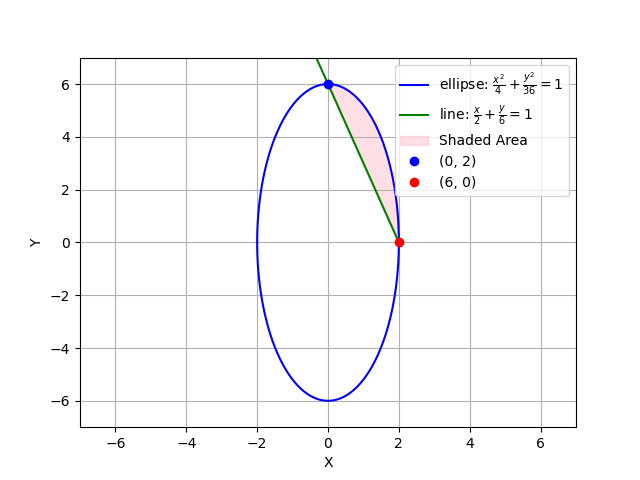
\includegraphics[width=0.7\columnwidth]{figs/fig.png}
    \caption{Area between line and ellipse}
\end{figure}
\end{document}
